\documentclass[unknownkeysallowed]{beamer}

\mode<presentation>
\usetheme{NCSUstat}
\setbeamercovered{transparent}
\usepackage[english]{babel}
\usepackage[latin1]{inputenc}
\usepackage{times}
\usepackage[T1]{fontenc}
\usepackage{booktabs}
\usepackage{subfig}
\usepackage{smartdiagram}
\RequirePackage{tikz}
\usepackage{bm}
\title[MS Thesis Defense] % (optional, use only with long paper titles)
{Application of EEG in User Verification}
\subtitle{Using Neurosky MindWave Mobile} % (optional)
\author[First Last] % (optional, use only with lots of authors)
{Pratheek~Bramhasamudra Mallikarjuna}
\institute[NCSU]
{
  Department of Electrical and Computer Engineering\\%Your Department Goes Here
  North Carolina State University
}
\NCSUupperline{\insertshorttitle}
\NCSUlowerline{\copyright{} \the\year{} by Pratheek Bramhasamudra Mallikarjuna}
%\subject{Statistical Theory and Methods}


%\date{} %% uncomment to leave out the date, or to use a specific date

%%%%%%%%%%%%%%%%%%%%%%%%%%%%%%%%%%%%%%%%%%%%%%%%%%%%%%%%%%%%%%%%%%%%%%
\begin{document}

\begin{frame}
  \titlepage
\end{frame}
%%%%%%%%%%%%%%%%%%%%%%%%%%%%%%%%%%%%%%%%%%%%%%%%%%%%%%%%%%%%%%%%%%%%%%
\begin{frame}{Outline}
\tableofcontents
\end{frame}

%%%%%%%%%%%%%%%%%%%%%%%%%%%%%%%%%%%%%%%%%%%%%%%%%%%%%%%%%%%%%%%%%%%%%%
\section{Introduction}

\subsection{Security}

\begin{frame}
	\frametitle{Security}
    Security is the procedure or measure taken to ensure safety.\\

    \pause
    \textbf{Types of security:}
    \pause
    \begin{enumerate}
    	\item Have something : ID card
    	\item Know something : User-name/Password
    	\item Be someone : Bio-metric identification
    \end{enumerate}
    \pause
    Some security systems use combination of these methods (For example, Military)	
\end{frame}

\subsection{EEG as a Security input}
\begin{frame}
	\frametitle{EEG as a Bio-metric Security}
    \begin{enumerate}
    	\item Different brain activities generate different brain waves
        \pause
        \item Harder to steal (unlike an ID card)
        \pause
        \item Harder to reproduce (unlike a fingerprint)
    \end{enumerate}
\end{frame}

\subsection{Problem Statement}
\begin{frame}
	\frametitle{Problem Statement}
    Evaluate the feasibility of using a single EEG input for Computer Security
\end{frame}

%%%%%%%%%%%%%%%%%%%%%%%%%%%%%%%%%%%%%%%%%%%%%%%%%%%%%%%%%%%%%%%%%%%%%%
\section{Background}

\subsection{EEG and EEG Bands}
\begin{frame}
  \frametitle{Electroencephalogram}
   Defined as (Mayo Clinic), ``A test that detects electrical activity in your brain using small, flat metal discs (electrodes) attached to your scalp''
  \begin{figure}[hbtp]
    	%\centering
    	\subfloat[EEG mesh]{
    		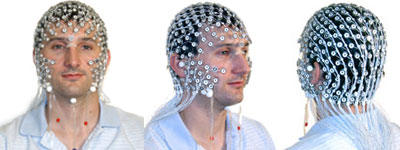
\includegraphics[width=0.4\textwidth]{EEG_mesh}
    	} \hspace{2cm}
    	\subfloat[MindWave]{
    		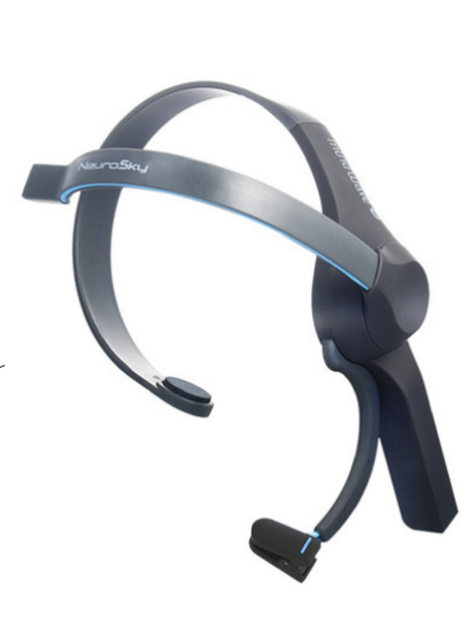
\includegraphics[width=0.2\textwidth]{mindwavemobile}
    	}
    	
    	\label{eeg_sensors}
    \end{figure}
\end{frame}

\begin{frame}
  \frametitle{EEG frequency bands}
    \begin{figure}[hbtp]
    	\centering
    	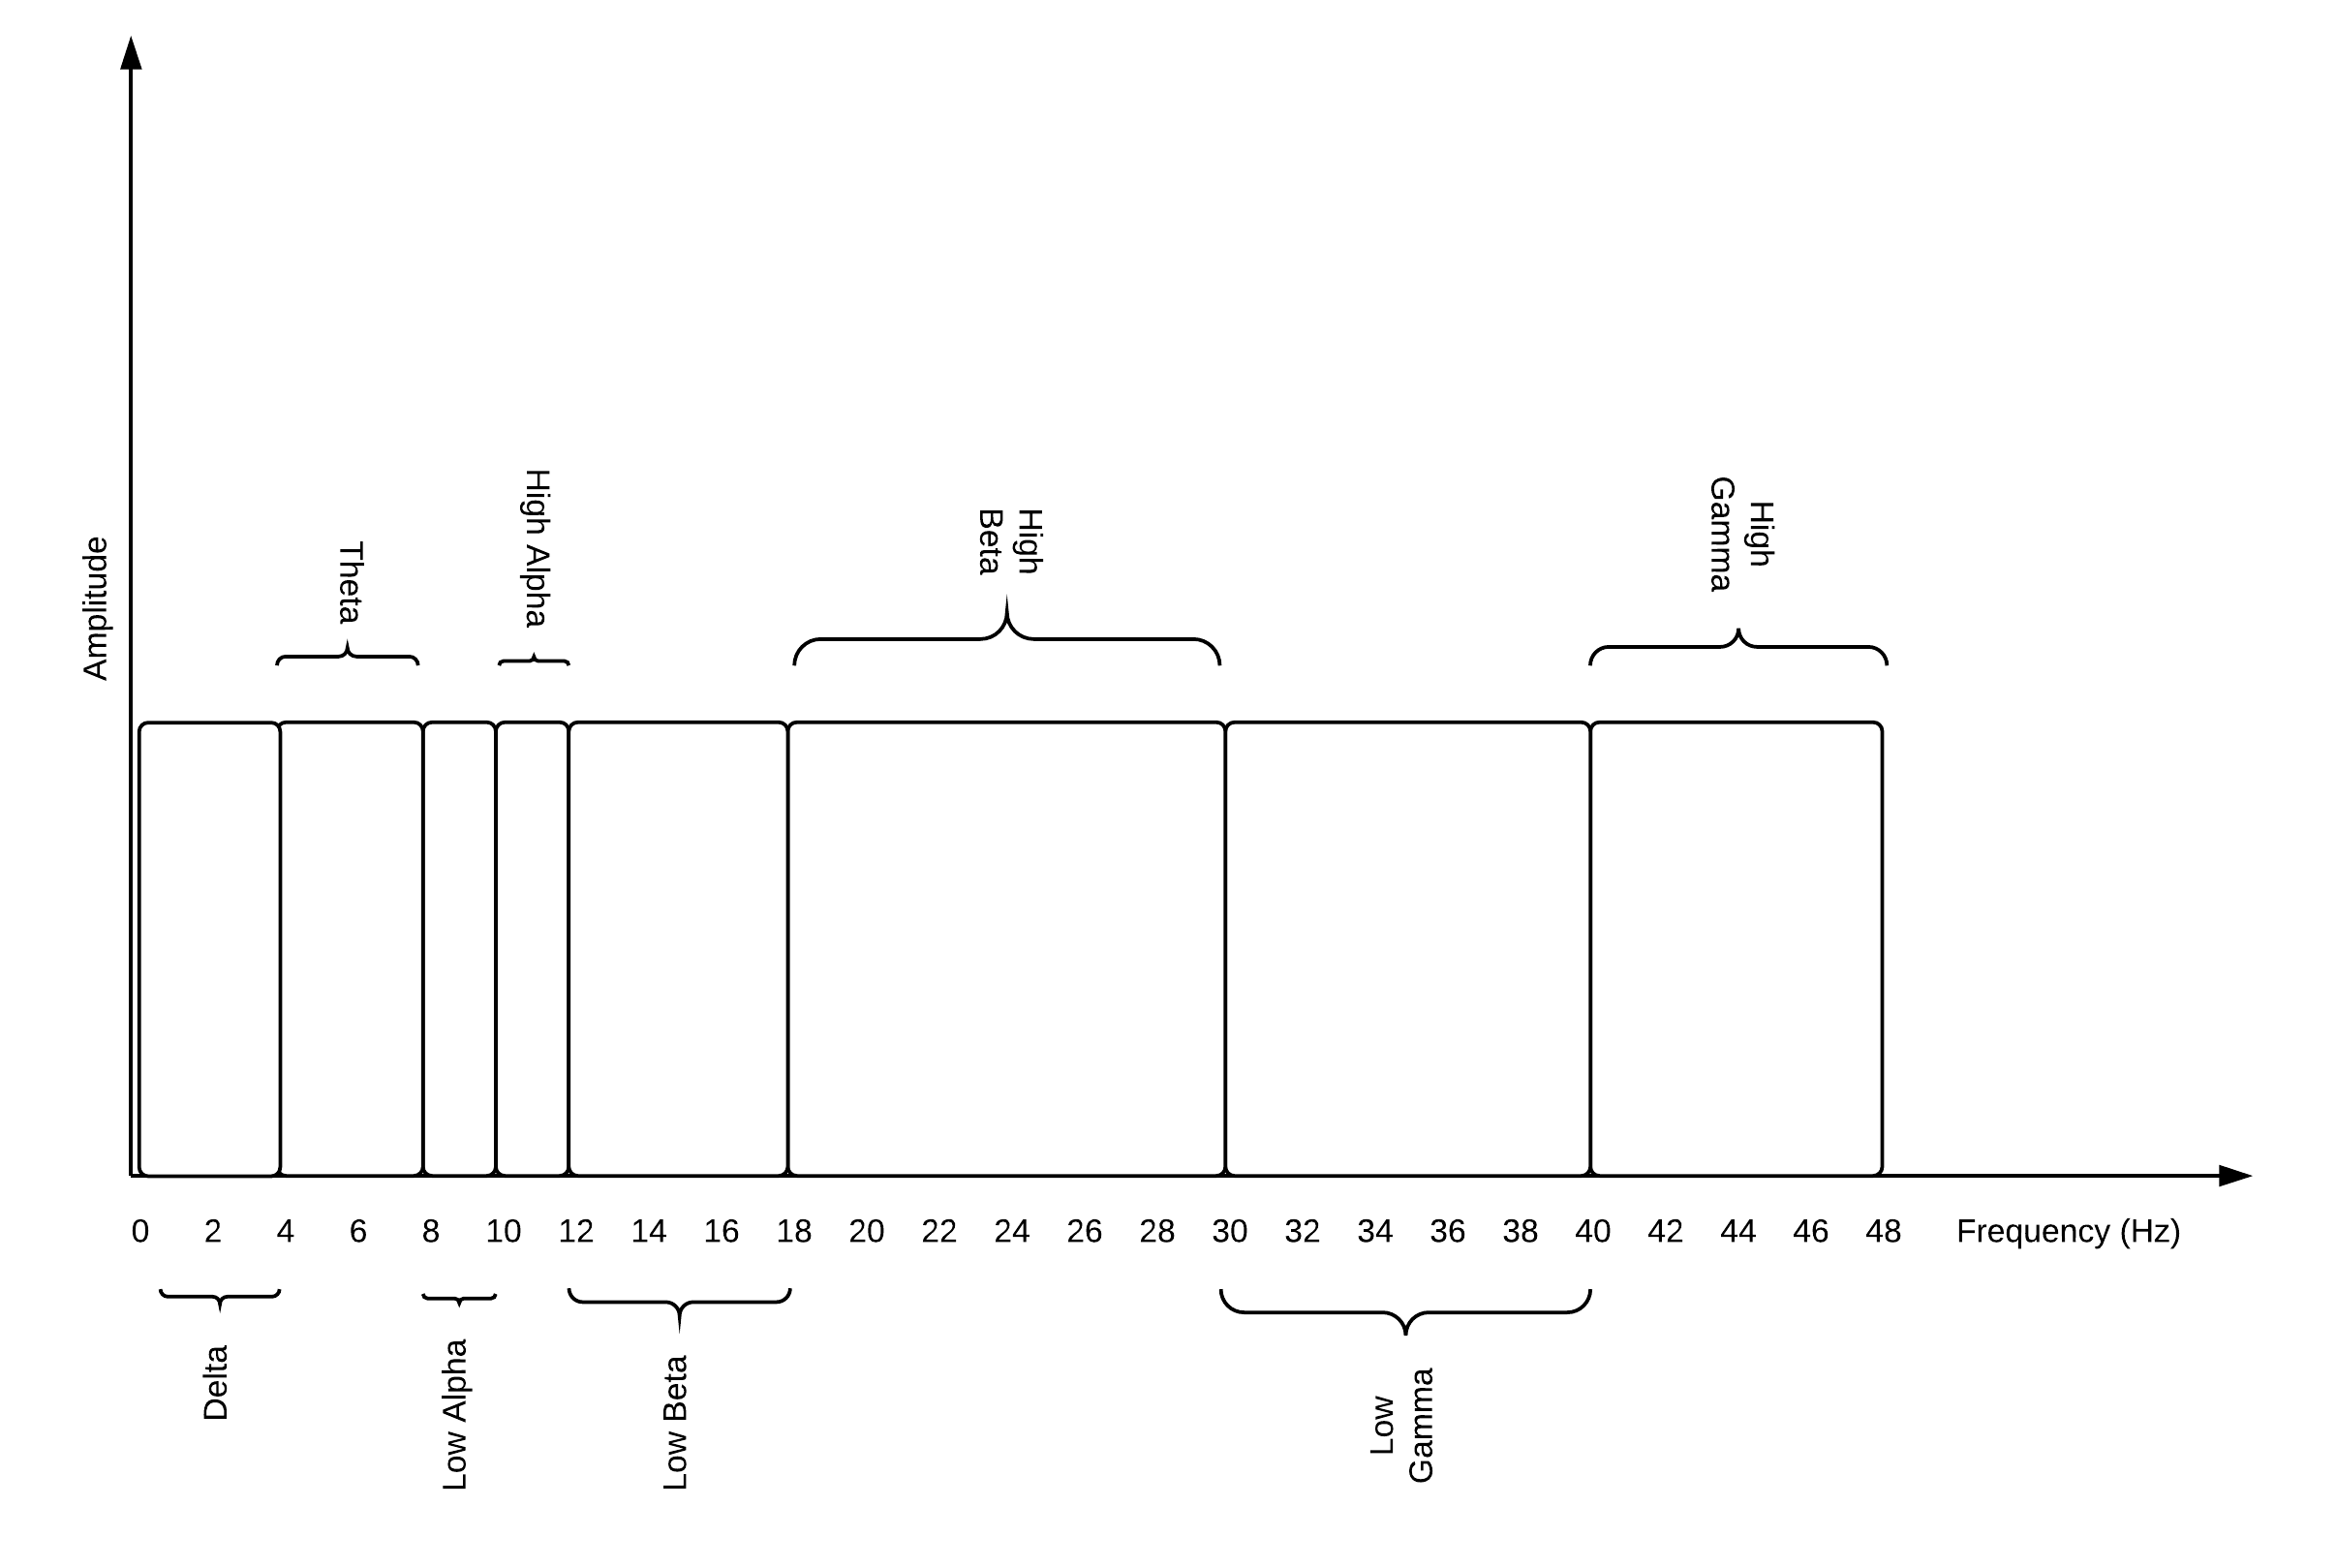
\includegraphics[width=0.9\textwidth]{EEG_bands}   	
    	\label{eeg_bands}
    \end{figure}  
\end{frame}

\begin{frame}
	\frametitle{EEG frequency bands cont.}
    	\begin{table}[h!]
		\centering
		\caption{Frequency Bands used for Feature extraction}
		\label{Table:Bands_more}
		\begin{tabular}{l l}
			\hline
			Name &Frequency Band\\\hline
			Delta&0.1Hz - 4Hz\\
			Theta&4Hz - 8Hz\\
            Low Alpha&8Hz - 10Hz\\
			High Alpha&10Hz - 13Hz\\
            Low Beta&13Hz - 18Hz\\
			High Beta&18Hz - 30Hz\\
            Low Gamma&30Hz - 40Hz\\
			High Gamma&40Hz - 48Hz\\
		\end{tabular}
	\end{table}
\end{frame}
\subsection{EEG sensors}
\begin{frame}
  \frametitle{Clinical vs Commercial EEG sensors}
  Clinical Sensors\\
  \pause
  \begin{enumerate}
    \item Hard  to set up
    \pause
    \item Expensive
    \pause
    \item More electrode, so more data
    \pause
  \end{enumerate}
  
  Commercial EEG sensors
  \pause
  \begin{enumerate}
    \item Easy  to set up
    \pause
    \item Cheaper 
    \pause
    \item Often fewer electrodes, so less data
  \end{enumerate}
\end{frame}

\section{EEG Verification System}

\begin{frame}
	\frametitle{EEG Verification System}
		\begin{figure}[hbtp]
            %\centering
            \resizebox{.4\linewidth}{!}{%
            \smartdiagram[priority descriptive diagram]{
                \centering
                EEG Sensor,
                Pre-processing (Filtering),
                Feature Extraction,
                Classification,
                Class Assignment}
                }
    		\caption{Overview of User Verification System using EEG}
    		\label{fig:FlowChart}
            
    	\end{figure}
\end{frame}

\subsection{Data Collection}
\begin{frame}
	\frametitle{Data Collection}
    EEG Data collected while subjects closed their eyes and relaxed muscle movements
    \pause
    \begin{enumerate}
    \item Calculating : Performing a mental calculation of two digit multiplication
    \pause
    \item Breathing : Concentrating on breathing
    \pause
	\item Singing : Mentally singing a song without actually singing out loud\\
    \end{enumerate}
\end{frame}
\subsection{Pre-processing}
\begin{frame}
	\frametitle{Pre-processing}
    \begin{enumerate}
    \item The raw EEG data is Band-pass filtered \\
    \pause
    \item Lower cutoff frequency : 0.1Hz - Removes DC frequency\\
    \pause
    \item Higher cutoff frequency : 50Hz - Removes frequencies beyond 50Hz
    \end{enumerate}

\end{frame}

\subsection{Feature Extraction}
\begin{frame}
	\frametitle{Feature Extraction}
	\begin{enumerate}
    \item It was discovered that EEG band energy varies with different brain activities
    \pause
    \item DFT ($X(k)$) of the pre-processed EEG data is computed
    \pause
	\item Spectral Energy of each EEG band is computed using $E_i = \sqrt{\frac{1}{m_2 - m_1 + 1} \sum_{k=m_1}^{k=m_2} \left | X(k) \right | ^2} \;$ where $m_2$ > $m_1$ and $k=[m_1,m_2] \in $ EEG frequency band $i$
    \pause
    \item Spectral energies of 8 EEG bands are arranged into a vector
    \pause
    \item This vector is normalized to removed the effects of electrode sensitivity w.r.t different subjects using $X_{n} = \frac{1}{\left | X_{in} \right |} X_{in}$
	\end{enumerate}
\end{frame}

\subsection{Classification}
\begin{frame}
	\frametitle{Intra-subject and Inter-subject Classification}
    \begin{enumerate}
		\item \textbf{Intra - Subject Classification} : Identifying a brain task in a set of brain tasks performed by a single subject.
        \pause
        \item \textbf{Inter - Subject Classification} : Identifying a subject in a set of subjects performing the same brain task.
	\end{enumerate} 
\end{frame}

\begin{frame}
	\frametitle{Classifiers}
    Following classifiers were used:
    \pause
    \begin{enumerate}
    \item Mahalanobis Distance Classifier
    \pause
    \item Neural Network Classifier
	\pause
   	\item Support Vector Machine Classifier
    \end{enumerate}
\end{frame}

\begin{frame}
	\frametitle{Mahalanobis Distance Classifier}
    \begin{enumerate}
    \item The classifier uses the distance between the class means weighted by variance (covariance in case of multi-dimensional vectors)
    \pause
    \item Can be computed using $D^2_x = (\mathbf{x} - E[\mathbf{x}])^T \bm{\Sigma}^{-1} (\mathbf{x} - E[\mathbf{x}])$, where $\bm{\Sigma} ^{-1}$ is the inverse of the covariance matrix $\Sigma$ and $E[\mathbf{x}]$ is the expected value of $\mathbf{x}$
    \end{enumerate}
    
    
\end{frame}

\begin{frame}
	\frametitle{Neural Network Classifier}
    \begin{enumerate}
      \item An \textit{Artificial Neuron} is defined as a sum-of-products operator which produces a weighted sum of its inputs and passes that sum though a non-linear function such as a limiter or a sigmoid
      \pause
      \item An Artificial Neural Network (ANN) consists of several of such interconnected artificial neurons
      \pause
    \end{enumerate}
    \small{
    \begin{table}[h!]
      \centering
      \caption{Neural Network Features}
      \label{NN_features}
      \begin{tabular}{l l}
      \hline
      Parameters &Value\\\hline
      Type of network &Feed Forward network\\
      Input layer size &8\\
      No. of hidden layers &1\\
      Hidden layer size &8\\
      Output layer size &Vary based on number of classes\\
      Activation function in hidden layer &Sigmoid\\
      Training Algorithm used &Backpropagation Algorithm
      \end{tabular}
    \end{table}}
\end{frame}

\begin{frame}
	\frametitle{Support Vector Machine Classifier (SVM)}
    \begin{enumerate}
    \item SVMs maximize the distance between the separating hyperplane and the nearest points of the classes to the hyperplane
    \pause
    \item SVMs preprocess the m-dimensional input vector to represent patterns in a n-dimension space - typically $n>>m$
    \pause
    \item Can perform non-linear classification using kernel functions (typically RBF kernels)
    \pause
    \item Suitable for binary classification, can perform multi-class classification using one-vs-all method
    \pause
    \item Not affected by curse of dimensionality
    \end{enumerate}
\end{frame}

\section{Results and Discussion}
\begin{frame}
	\frametitle{Intra-subject Classification}
        \begin{figure}[hbtp]
    	\centering
    	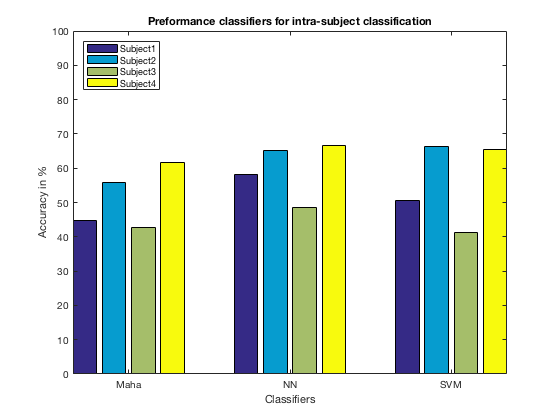
\includegraphics[width=0.7\textwidth]{base_total_all}   	
    	\label{Intra-Subject classification}
    \end{figure} 
\end{frame}

\begin{frame}
	\frametitle{Inter-subject Classification}
     \begin{figure}[hbtp]
    	\centering
    	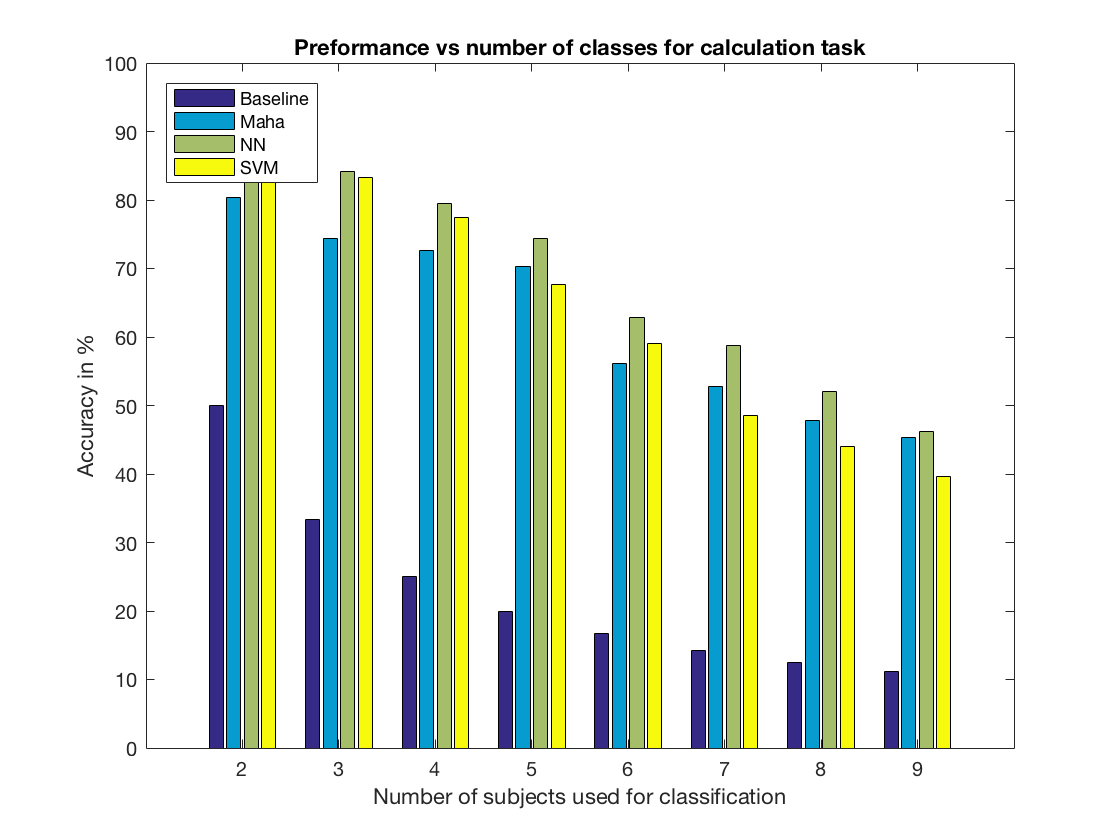
\includegraphics[width=0.7\textwidth]{calc_base}   	
    	\label{Inter-Subject classification for calculation}
    \end{figure} 
\end{frame}

\subsection{Conclusion and future work}
\begin{frame}
	\frametitle{Conclusion and future work}
    \begin{enumerate}
    \item Intra-subject accuracies are low. Possible reason : similarities in brain waves from same subject performing different tasks
    \pause
    \item Identifying certain tasks are easier compared to other (calculation)
    \pause
    \item Performance of inter-subject classification drops with increase in number of subjects and thus it is not scalable
    \pause
    \item Quantification of level of training needed for the humans could be a future work
    \end{enumerate}
\end{frame}

\subsection{Questions?}
\begin{frame}
	\frametitle{Questions?}
\end{frame}

\section{Demo}
\begin{frame}
	\frametitle{Demo}
\end{frame}
\end{document}
